\section{Bestimmung des hadronischen Wirkungsquerschnitts $\sigma_0^{Had}$}
\subsection{Selektion der hadronischen Ereignisse}
Wir haben mehrere Datensamples zu Verfügung gehabt. Zunächst waren dort die gemessenen L3-Daten, die bei verschiedenen Schwerpunktenergien aufgenommen wurden (bei 89.48 GeV, 91.33 GeV und 93.02 GeV). Die integrierten Luminositäten unterscheiden sich auch und wurden in \cite[S.9]{script} gegeben; außerdem konnten wir mit zwei Monte-Carlo-Daten (MC) arbeiten, die uns der aktuellen Theorie entsprechende Verteilungen von Hadronen und Myonen gab. Mit diesen Simulationsdaten konnten wir also überprüfen, welche Wirkung unsere Cuts auf den jeweiligen $Z^0$-Zerfallskanal hatten. So konnten wir feststellen, dass bei hadronischen Ereignissen immer mindestens ca. 9 Cluster (separierte Einträge im Kalorimeter) Teilchen detektiert haben (siehe \fref{Ncluster_vgl}).
\begin{figure}[htb]
	\centering
	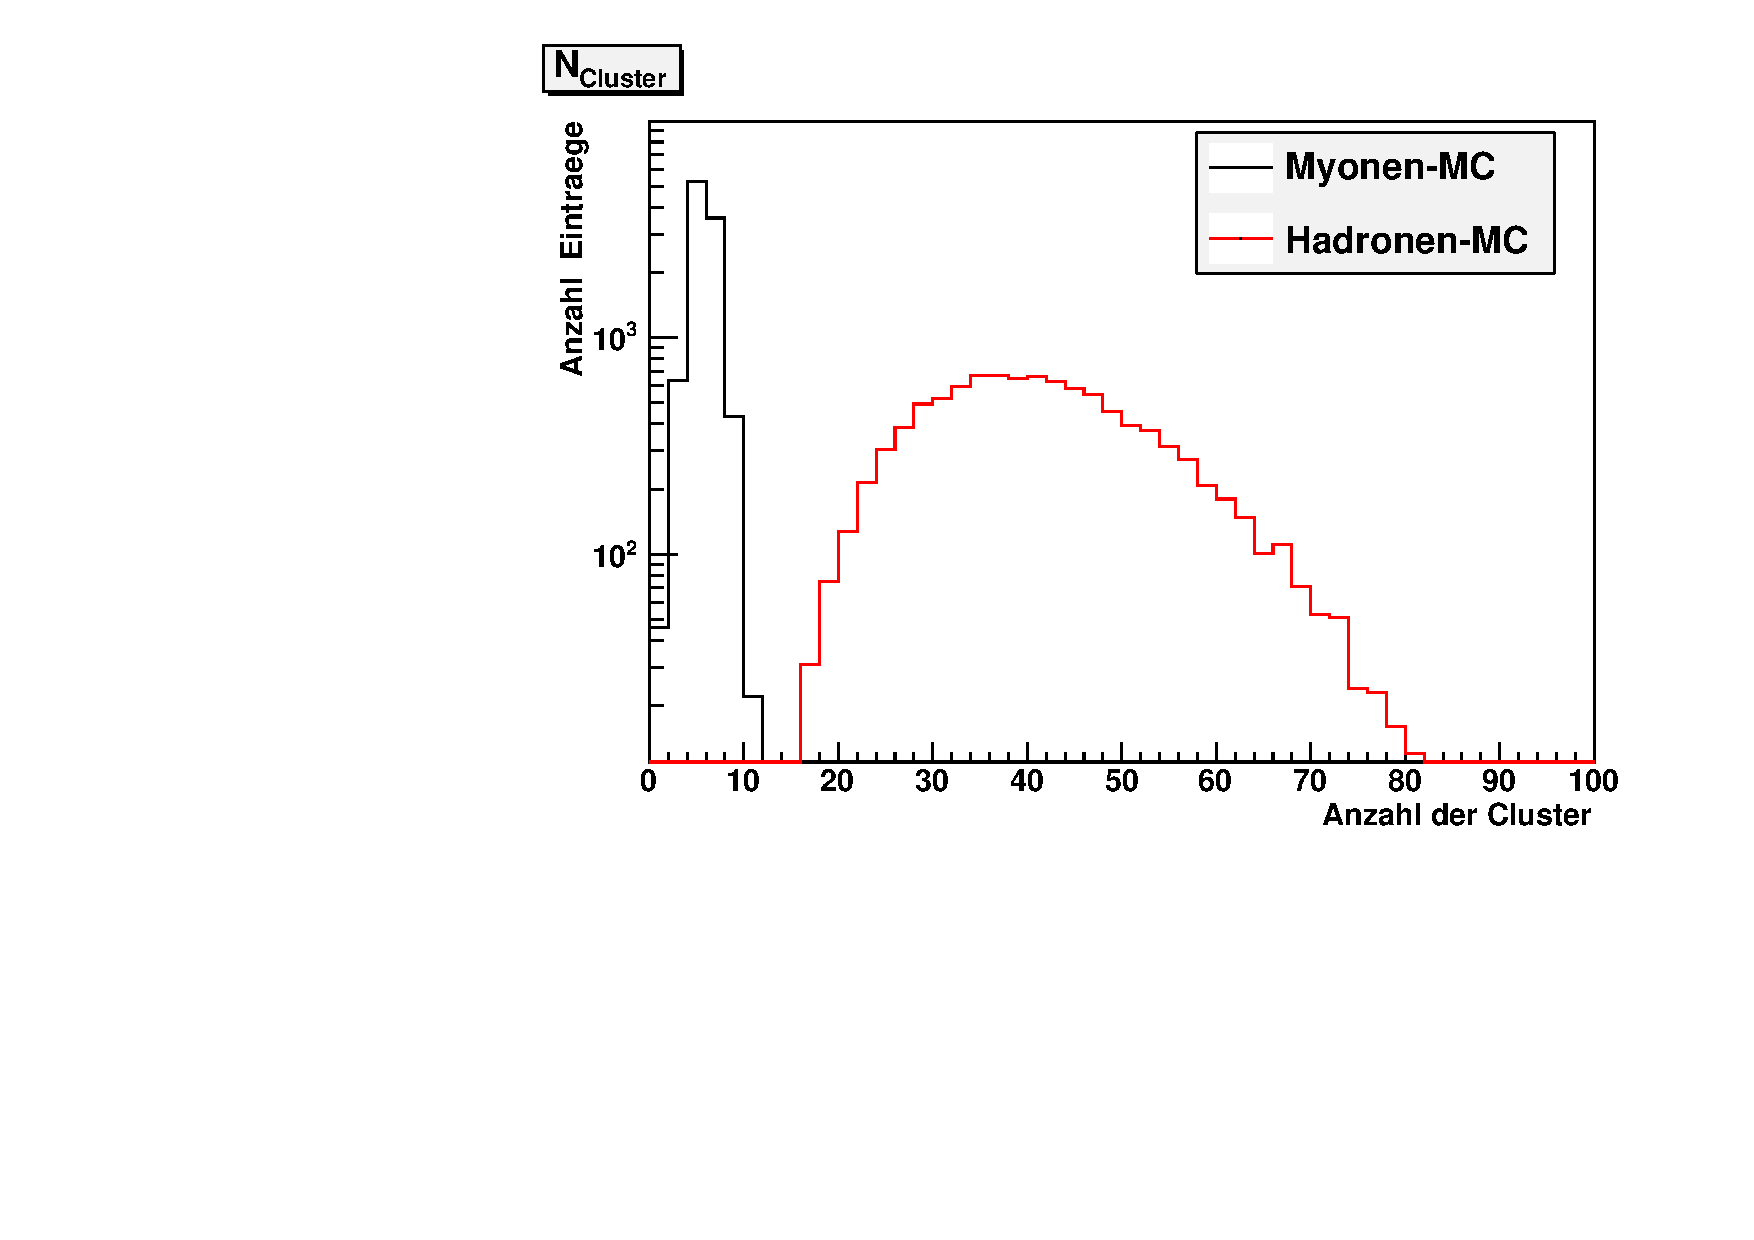
\includegraphics[width=1\columnwidth,keepaspectratio]{Ncluster_vgl.pdf}
	\caption{Verteilung der Kalorimetereinträge für MC-Samples}
	\label{fig:Ncluster_vgl}
\end{figure}
Daraus ließ sich ein wirksamer Cut gewinnen, der unter anderem die meisten Myonen-Ereignisse nicht zulässt. Ein weiterer Cut wurde angewendet, indem verlangt wurde, dass die (sichtbare) Energie eines Events mehr als $70\%$ der Schwerpunktsenergie beträgt (siehe \fref{Evisvgl_mc} für einen Vergleich der sichtbaren Energie für beide MC-Samples).
\begin{figure}[htb]
	\centering
	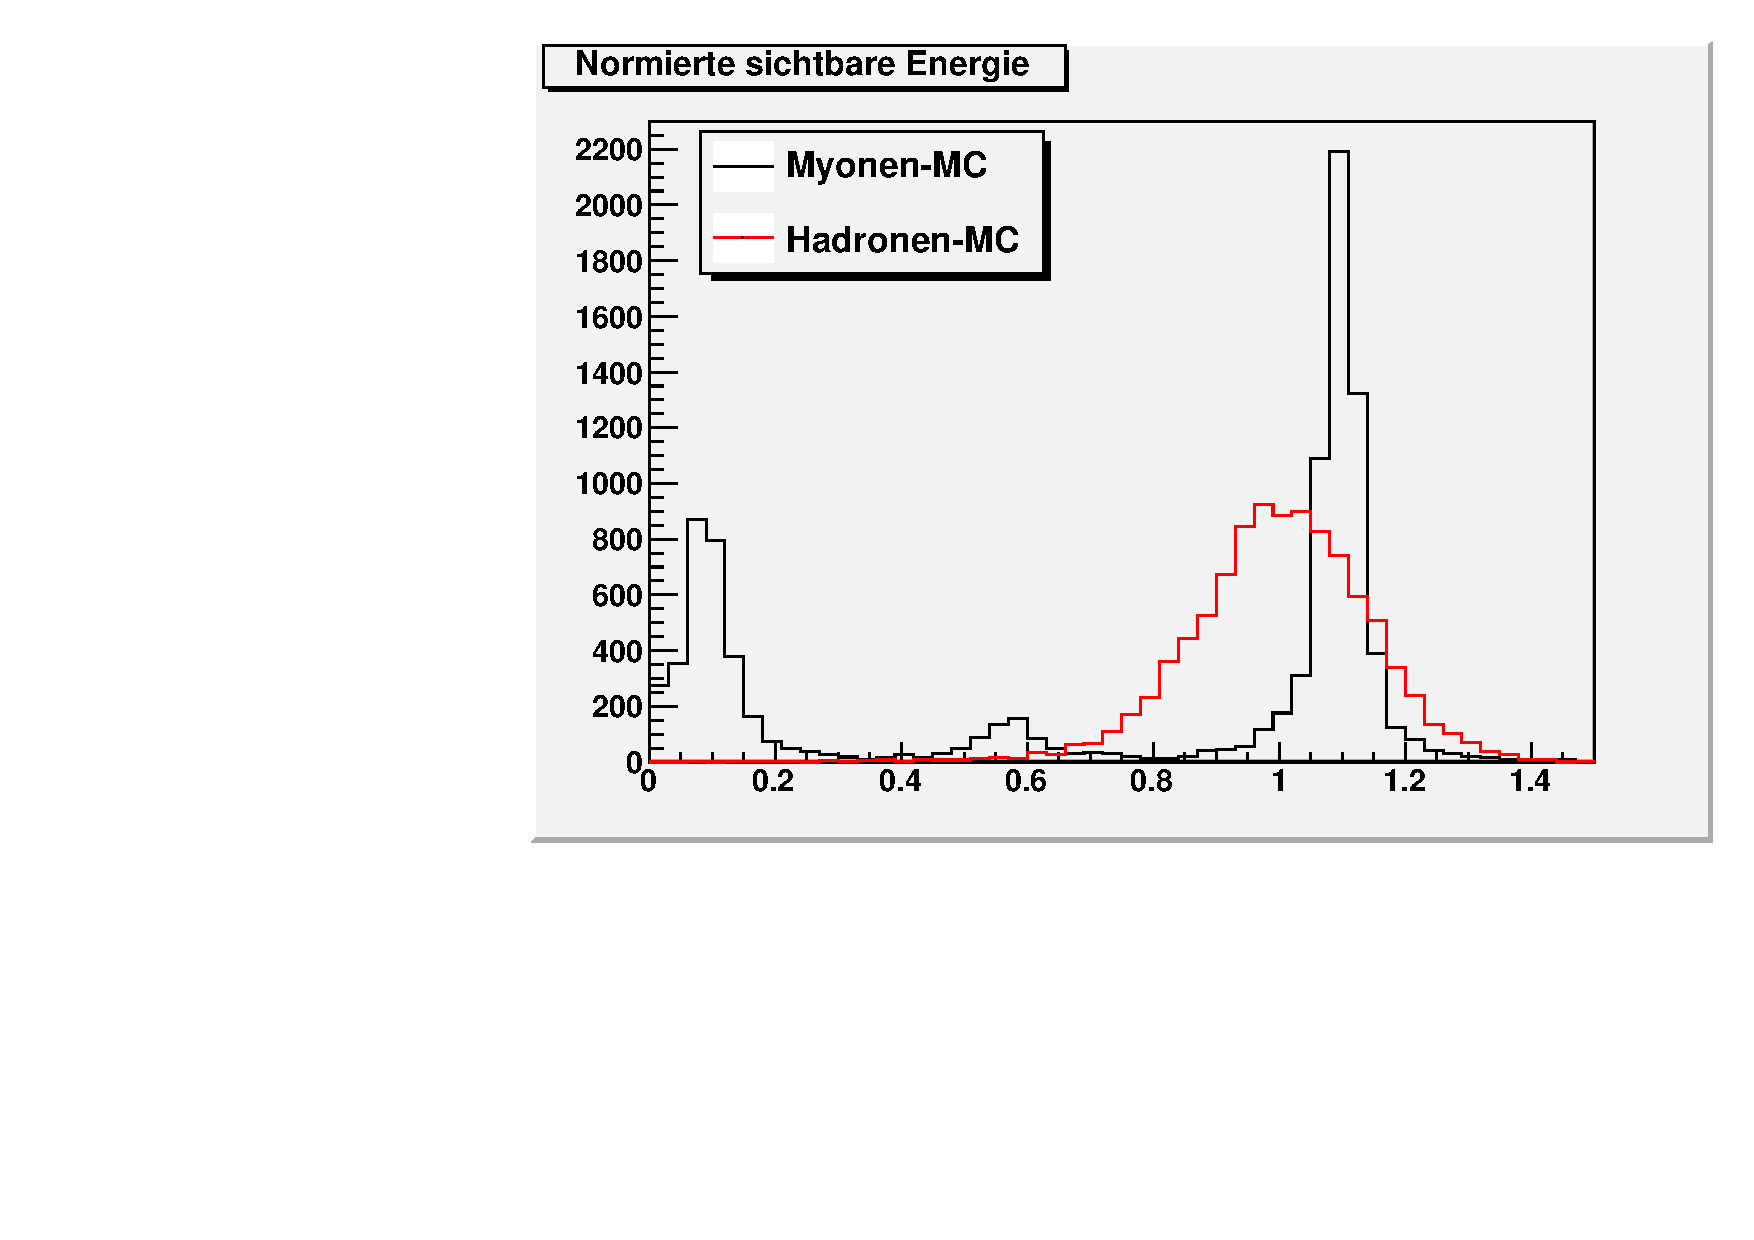
\includegraphics[width=1\columnwidth,keepaspectratio]{Evisvgl_mc.pdf}
	\caption{Verteilung der sichtbaren Energie für MC-Samples}
	\label{fig:Evisvgl_mc}
\end{figure}
Zum Beispiel zerfallen $\tau$-Leptonen oft so, dass die Art und Anzahl der Teilchen, die in die Kalorimeter gelangt, sehr einem hadronischen Ereignis ähnelt. Allerdings wird dabei viel Energie an dabei entstehende Neutrines abgegeben, die nicht registriert werden können, sodass die sichtbare Energie in einem solchen Fall wesentlich kleiner ist. Mit diesem Cut können demnach viele $\tau$-Zerfälle ausgeschlossen werden. Dabei haben wir auch immer darauf geachtet, dass die Effizienz unserer Cuts nicht zu klein wird. Mit den eben erwähnten Cuts gelang es uns, eine Effizienz von
\begin{eqnarray}
\epsilon_{had} &=& \frac{9770 \pm \sqrt{9770} \pm 158}{10000}\\
&=& 0.98 \pm 0.01 \pm 0.02
\end{eqnarray}
zu erreichen. Dabei ist der erste angegebene Fehler der statistische Fehler und der zweite ist der systematische Fehler, der aus der ''willkürlichen'' Wahl der Schnittkriterien resultiert. Wenn man diese Cuts allerdings auf das Myonen-Monte-Carlo-Sample anwendet, so werden nur 19 hadronische Events erkannt (bei 9970 Events im Sample!). Die Fehlerquote durch Myonenereignisse ist also sehr gering. Unsere Schnitte sind also offenbar gut geeignet, um Hadronen-Events aus den Daten zu selektieren.

\subsection{Berechnung der hadronischen Wirkungsquerschnitte bei verschiedenen $\sqrt{s}$}
Die eben besprochenen Schnitte haben wir nun auf die Messdaten angewandt. Dabei kamen die in \tref{hadronic_xsecs} gezeigten Werte heraus. Die angegebenen Fehler sind wiederum statistischer und dann systematischer Fehler. Diese Konvention verwenden wir im gesamten folgenden Protokoll.\\
Der Fehler des Wirkungsquerschnitts ergibt sich durch Fehlerfortpflanzung aus den jeweiligen Fehlern von N und von $\epsilon_{had}$.
\begin{figure*}
\begin{tabular*}{\textwidth}{%
S[tabformat=2.1]%
l%
l}
\toprule
{Energie [\si{GeV}]} &
{Zahl analysierter Hadr.-Ereignisse N} &
{Wirkungsquerschnitt $\sigma_0^{Had}$ [\si{\nano\barn}]}\\
\midrule
89,48 & 1848 ± 43 ± 52 & 10,55 ± 0,18 ± 0,16 \\
91,33 & 3980 ± 63 ± 79 & 29,98 ± 0,49 ± 0,43 \\
93,02 & 2149 ± 46 ± 51 & 14,56 ± 0,24 ± 0,24 \\
\bottomrule
\label{tab:hadronic_xsecs}
\end{tabular*}
\caption{Zahl der analysierten Hadronen-Ereignisse und zugehörige Wirkungsquerschnitte bei verschiedenen Schwerpunktsenergien}
\end{figure*}

Der Wirkungsquerschnitt, der auch in \tref{hadronic_xsecs} aufgeführt ist, ergibt sich aus den gegebenen Daten nach \cite[Gl.13]{script} wie folgt:
\begin{eqnarray}
\sigma_{had} = \frac{N - N_U}{L\epsilon_{had}} = \frac{N}{L\epsilon_{had}}
\end{eqnarray}
$N$ ist dabei die Zahl der analysierten Hadronenereignisse, $L$ ist die bereits erwähnte schwerpunktsenergieabhängige Luminosität und $\epsilon_{had}$ wurde oben bereits eingeführt. Die Zahl der vermuteten Untergrundereignisse $N_U$ haben wir auf null gesetzt, weil unsere Cuts die jeweiligen Events sehr effektiv passieren lassen. Außerdem kann man die Form der Verteilungen von z.B. der sichtbaren Energie (nach den betreffenden Selektionsschnitten) sowohl für die Monte Carlo-Samples wie auch für die Daten-Samples vergleichen (\fref{Evis_vgl}).
\begin{figure}[htb]
	\centering
	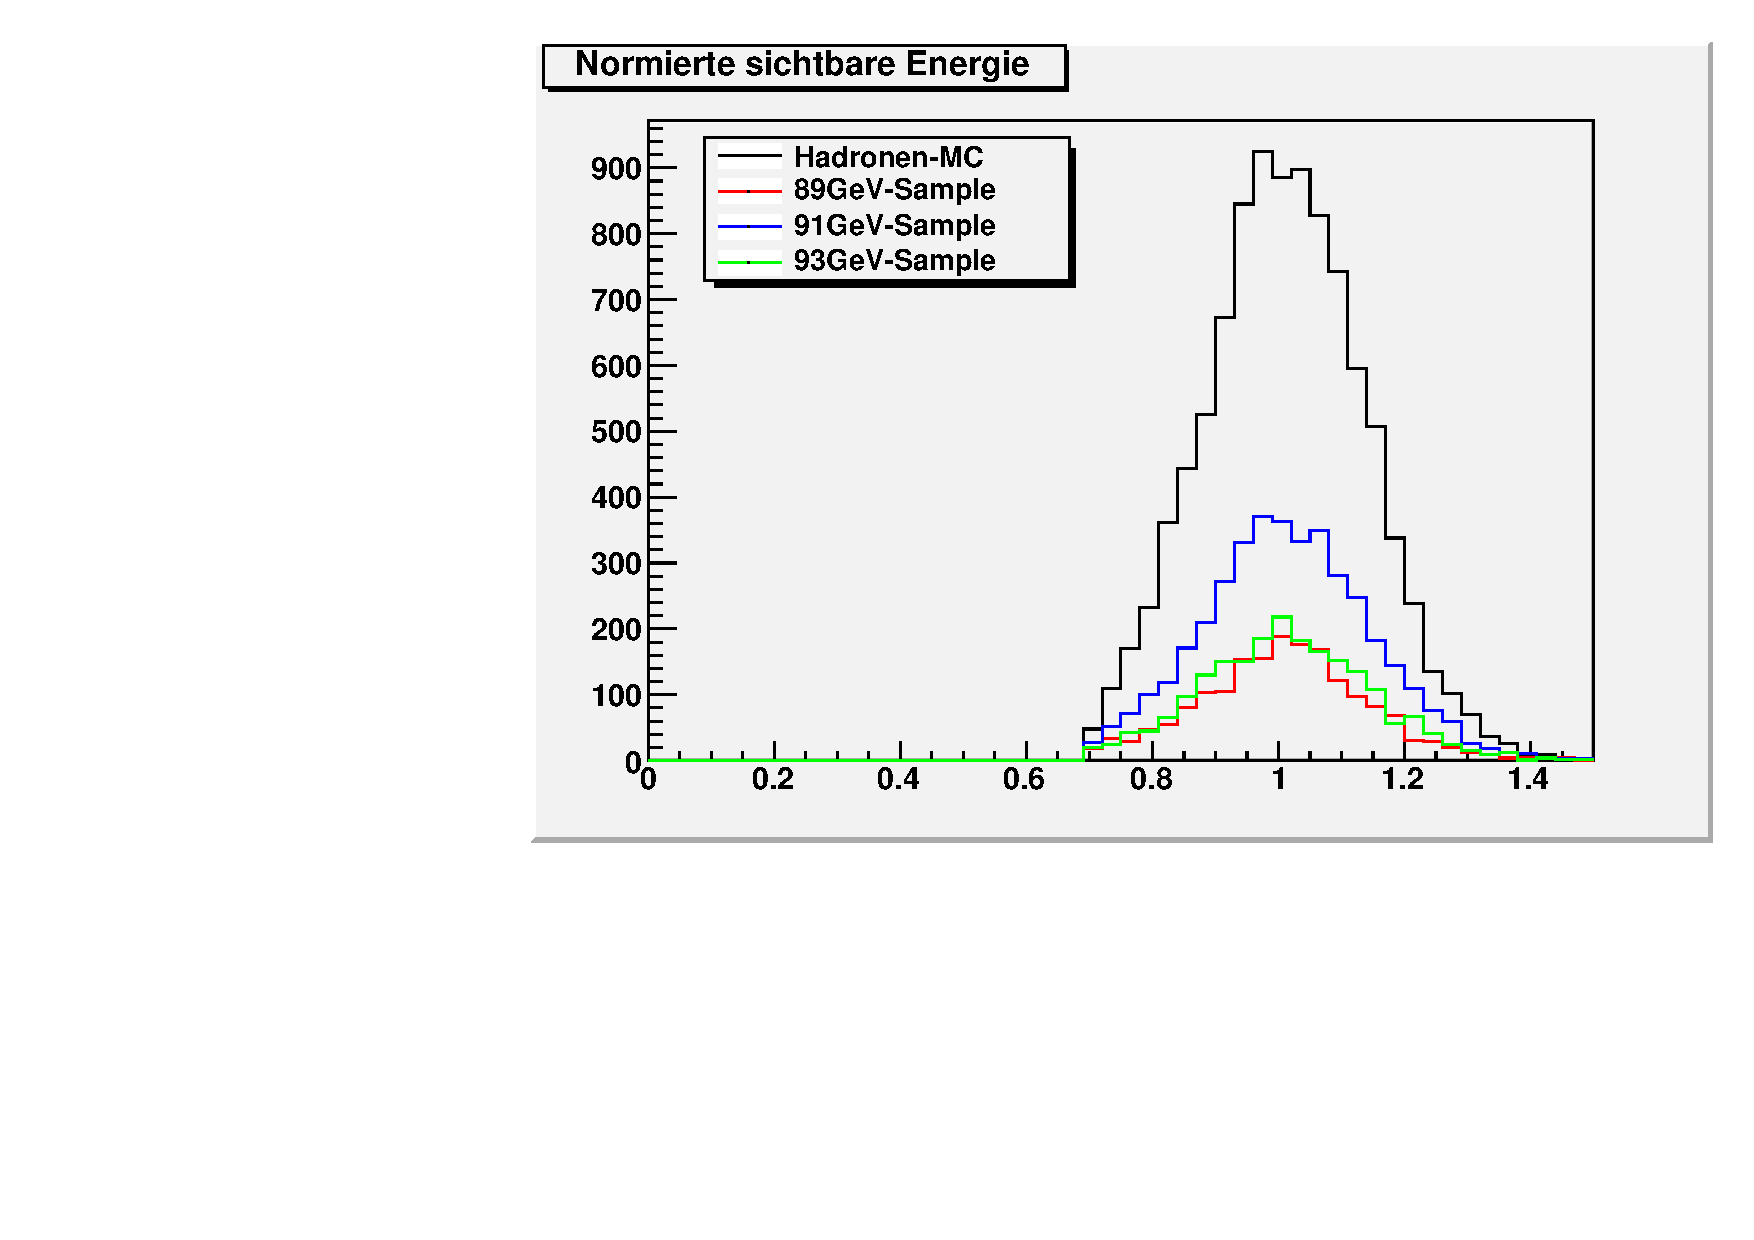
\includegraphics[width=1\columnwidth,keepaspectratio]{Evis_vgl.pdf}
	\caption{Verteilung der sichtbaren Energie für verschiedene Samples}
	\label{fig:Evis_vgl}
\end{figure}
Wie man sehen kann, sehen sich die Verteilungen sehr ähnlich, was die Vermutung nahelegt, dass vornehmlich die gleichen Prozesse stattfanden. Dies bestätigt uns in der Annahme, dass der Untergrund mit gutem Gewissen vernachlässigt werden kann.\\
Der statistische Fehler des Wirkungsquerschnitts ergibt sich durch Fehlerfortpflanzung aus den jeweiligen Fehlern von $N$, $L$ und $\epsilon_{had}$:
\begin{eqnarray}
\Delta\sigma_{had} &=& \sqrt{\left( \frac{\partial\sigma}{\partial L}\Delta L\right)^2 + \left( \frac{\partial\sigma}{\partial N}\Delta N\right)^2 + \left( \frac{\partial\sigma}{\partial \epsilon_{had}}\Delta\epsilon_{had} \right)^2}\\
&=& \sqrt{\left( \frac{N}{L^2\epsilon_{had}}\Delta L\right)^2 + \left( \frac{1}{L\epsilon_{had}}\Delta N\right)^2 + \left( \frac{N}{L \epsilon_{had}^2}\Delta\epsilon_{had} \right)^2}
\end{eqnarray}
In dieser Art haben wir auch alle weiteren Fehler berechnet, wie z.B. den systematischen Fehler von $\sigma_{had}$, der sich aus den systematischen Unsicherheiten von $N$ und $\epsilon_{had}$ zusammensetzt.

Diese Wirkungsquerschnitte kann man nun in das bereitgestellte Fit-Programm einsetzen. Dieses Programm wurde von uns leicht verändert und kann im Anhang unter \lref{fit} gefunden werden. Unter Berücksichtigung der statistischen Fehler von N, $\epsilon_{had}$ und der Luminosität (deren Fehler war in \cite[S.9]{script} mit $1\%$ des gegebenen Wertes angegeben) kann der statistische Fehler von $\sigma_0$ und mit den systematischen Fehlern von N und $\epsilon_{had}$ durch dieses Programm berechnet werden. Für den gesamten hadronischen Wirkungsquerschnitt resultiert also:
\begin{eqnarray}
\sigma_0^{Had} = 40.33 \pm 0.65 \pm 0.27
\end{eqnarray}
Der Gesamtfehler, der pythagoräisch aus dem systematischen und dem statistischen Fehler addiert wird, beträgt ungefähr $2\%$ des Absolutwertes.

\section{Bestimmung des myonischen Wirkungsquerschnitts $\sigma_0^{Mu}$}
\subsection{Selektion der Myonenereignisse}
Hier sind wir genauso wie bei der Selektion der Hadronenevents vorgegangen. Wie bereits oben in \fref{Ncluster_vgl} gezeigt, haben alle Myonen-Ereignisse weniger als 12 Cluster-Einträge, was als Cut genutzt wurde. Weiterhin konnte man anhand der Masse verlangen, dass mindestens zwei Teilchen die Masse eines Myons besitzen. Außerdem sollte der Kosinus des Winkels, den die Bahnen beider Myonen bilden, größer als 0.9 sein, da man verlangen möchte, dass die Myonen annähernd Back-to-Back fliegen sollten. Schließlich haben wir an die Energie eines Events einige Anforderungen gestellt, zum Beispiel, dass eines der Myonen ca. die Hälfte der Gesamtenergie trägt. Die Ideen für diese Cuts kamen im Wesentlichen aus ??BLABLA?? (Kap. 5). Mit diesen Schnitten erhielten wir eine Effizienz von
\begin{eqnarray}
\epsilon_{Mu} &=& \frac{5855 \pm sqrt{5855} \pm 197}{9970} = 0.59 \pm 0.01 \pm 0.02
\end{eqnarray}
Damit konnten, analog zum Hadronen-Fall, die Wirkungsquerschnitte bei den verschiedenen Schwerpunktsenergien angegeben werden. Die Ergebnisse sind in \tref{muonic_xsecs} zu finden.
\begin{figure*}
\begin{tabular*}{\textwidth}{%
S[tabformat=2.1]%
l%
l}
\toprule
{Energie [\si{GeV}]} &
{Zahl analysierter Myonen-Ereignisse N} &
{Wirkungsquerschnitt $\sigma_0^{Mu}$ [\si{\nano\barn}]}\\
\midrule
89,48 & 67 ± 8 ±  & 10,55 ± 0,18 ± 0,16 \\
91,33 & 122 ± 11 ± 79 & 29,98 ± 0,49 ± 0,43 \\
93,02 & 77 ± 9 ± 51 & 14,56 ± 0,24 ± 0,24 \\
\bottomrule
\label{tab:muonic_xsecs}
\end{tabular*}
\caption{Zahl der analysierten Myonen-Ereignisse und zugehörige Wirkungsquerschnitte bei verschiedenen Schwerpunktsenergien}
\end{figure*}

\subsection{Bestimmung des Wirkungsquerschnitts}